\section{Beleg}

\begin{exercise}
    Sei $G\setleq \reals^n$ nicht leer und durch
    $$
    G=\set{x\in\reals^n:g(x)\leq 0, h(x)=0},
    $$
    wobei $g:\reals^n\to\reals^m$ und $h:\reals^n\to\reals^l$ stetig differenzierbare Funktionen seien. Für einen Punkt $x\in G$ ist der \keyword{Kegel der zulässigen Richtungen} definiert durch
    $$
    Z(X):=\set{d\in R:\exists t>0:\forall s\in[0,t]:g(x+sd)\leq 0, h(x+sd)=0}. 
    $$
    Weiter sei der \keyword{Linearisierungskegel} gegeben durch
    $$
    L(x):=\set{d\in\reals^n:g_i'(x)d\leq 0,\forall i\in I_0(x), h'(x)d=0},
    $$
    wobei $I_0(x)$ die Indexmenge der in $x$ aktiven Richtungen bezeichne, d.h.
    $$
    I_0(x):=\set{i\in m: g_i(x)=0}.
    $$
    \begin{tasks}
            \item Skizzieren Sie die folgenden Bereiche $G\setleq \reals^2$ und geben Sie für $x=0$ jeweils $Z(x)$ und $L(x)$ an.
        \begin{tasks}
                \item $G=\set{x\in\reals^n: x_1\geq 0, x_2\geq 0, x_1^2+4x_2^2\leq 4}$,
                \item $G=\set{x\in\reals^2: x_1^2-x_2\leq 0, -x_1+x_2^2\leq 0}$,
                \item $G=\set{x\in\reals^2:x_1^2+{(x_2-1)}^2=1}$.  
        \end{tasks}
            \item Zeigen Sie, dass für jeden Punkt $x\in G$ gilt: $\cl(Z(x))\setleq L(x)$, wobei $\cl$ den topologischen Abschluss bezeichne.
        \item Die Funktionen $g_1,\ldots,g_m$ seien konvex und es existiere ein Punkt $y\in G$ mit $g_i(y)<0$ für $i=1,\ldots,m$. Ferner sei $h$ affin. Zeigen Sie dass dann $\cl(Z(x))=L(x)$ für $x\in G$.
    \end{tasks}
\end{exercise}

\begin{solution}
    \begin{tasks}
        \item Man erhält die folgenden Zeichnungen.
    \definecolor{gray}{rgb}{0.9,0.9,0.9}
        \begin{figure}[htb]
            \centering
            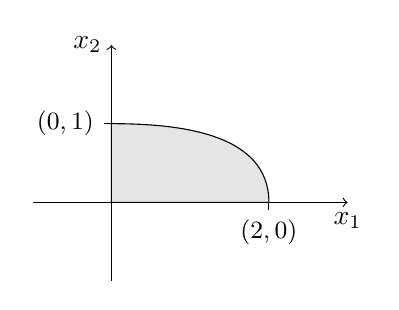
\begin{tikzpicture}
                % axis
                \draw[->] (-1,0) -- (3,0) node[anchor=north] {$x_1$};
                \draw[->] (0,-1) -- (0,2) node[anchor=east] {$x_2$};
                \draw[-] (2,0) -- (2,-0.1) node[anchor=north] {\small $(2,0)$};
                \draw[-] (0,1) -- (-0.1,1) node[anchor=east] {\small $(0,1)$};
                % area G
                \draw[fill=gray] (0,0) -- (2,0) to [out=90, in=0] (0,1)  to [out=-90, in=90] (0,0);
            \end{tikzpicture}
            \caption{(a) Viertelellipse, $Z(x)=L(x)={[0,\infty)}^2$.}
        \end{figure}
        \begin{figure}[htb]
            \centering
            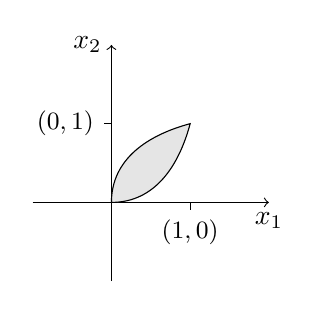
\begin{tikzpicture}
                % axis
                \draw[->] (-1,0) -- (2,0) node[anchor=north] {$x_1$};
                \draw[->] (0,-1) -- (0,2) node[anchor=east] {$x_2$};
                \draw[-] (1,0) -- (1,-0.1) node[anchor=north] {\small $(1,0)$};
                \draw[-] (0,1) -- (-0.1,1) node[anchor=east] {\small $(0,1)$};
                % area G
                \draw[fill=gray] (0,0) to [out=0, in=-105] (1,1) to [out=-165, in=90] (0,0);
            \end{tikzpicture}
            \caption{(b) Schnitt von zwei parabolisch betrenzten Mengen, $Z(x)={(0,\infty)}^2$, $L(x)={[0,\infty)}^2$.}
        \end{figure}
        \begin{figure}[htb]
            \centering
            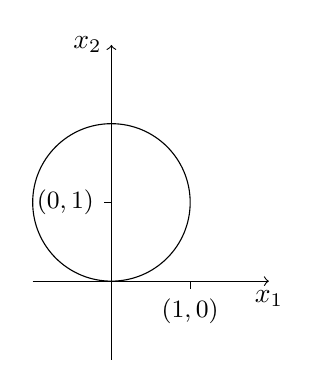
\begin{tikzpicture}
                % axis
                \draw[->] (-1,0) -- (2,0) node[anchor=north] {$x_1$};
                \draw[->] (0,-1) -- (0,3) node[anchor=east] {$x_2$};
                \draw[-] (1,0) -- (1,-0.1) node[anchor=north] {\small $(1,0)$};
                \draw[-] (0,1) -- (-0.1,1) node[anchor=east] {\small $(0,1)$};
                % circle G
                \draw (0,1) circle (1);
            \end{tikzpicture}
            \caption{(c)Kreis, $Z(x)=\emptyset$, $L(x)=\reals\settimes 0$.}
        \end{figure}     
        \item Sei $d\in\cl(Z(x))$, dann existiert for alle $\epsilon>0$ ein  Punkt $d'\in Z(x)$ mit $\norm{d-d'}<\epsilon$.
    Wir haben dann,
    $$
g_i'(x)d'\leq 0, h_j'(x)d'=0
$$
for $i\in I_0$, $j=1,\ldots,l$. Wir haben nun $g_i'(x)d\leq g_i'(x)(d-d')\leq \epsilon \norm{g_i'(x)}$. Damit folgt $g_i'(x)d\leq 0$. In analoger Weise erhält man $\abs{h_i'(x)d}=\abs{h_i'(x)(d-d')}\leq \epsilon\norm{h_i'(x)}$. Also $d\in L(x)$.
    \item Ohne Einschränkung können die $h_i$ weggelassen werden, indem wir uns auf den affinen Unterraum $\bigmeet_{i=1}^l{\ker{h_i}}$ beschränken (oder, indem wir die Gleichungsbedingungen durch je zwei Ungleichungsbedingungen ausdrücken, durch lineare, also konvexe Funktionen). Sei also $d\in L(x)$, dann gilt
$$
g_i'(x)d\leq 0
$$
für $i\in I_0(x)$. Ist die strikte Ungleichung erfüllt, so ist unmittelbar klar (aus der \person{Weierstraß}'schen Formel), dass $x\in Z(x)$. Wir dürfen also von Gleichheit ausgehen. In diesem Falle ist $\lambda \mapsto g_i(x+\lambda (y-x))$ konvex und wir haben
$$
g_i'(x)(d+\epsilon(y-x))=\epsilon g_i'(x)(y-x)\leq \epsilon g(y)<0
$$
für $\epsilon>0$. Damit liegen aber alle $d+\epsilon(y-x)$ aufgrund derselben Argumentation wie oben (\person{Weierstraß}'sche Formel) in $Z(x)$. Also liegt $d$ in dessen Abschluss.
    \end{tasks}
\end{solution}
